% !TeX root = ../tfg.tex
% !TeX encoding = utf8
%
%*******************************************************
% Introducción
%*******************************************************

% \manualmark
% \markboth{\textsc{Introducción}}{\textsc{Introducción}}

\chapter{Introducción}

\section{Contexto}

El desarrollo humano ha sido constantemente impulsado por avances tecnológicos que
han redefinido nuestra comprensión e interacción con mundo. Desde la invención
de la imprenta hasta la revolución digital actual, cada era ha estado marcada por
innovaciones clave. En particular, la invención de los ordenadores y el avance de
las tecnologías de la información han convergido en la capacidad de generar,
almacenar y analizar grandes volúmenes de datos. Este volumen de información ha desencadenado
lo que ahora conocemos como la Era de la Información, que se caracteriza por el
desarrollo de algoritmos avanzados que extraen valor de estos datos de manera
automática y eficiente.

Dentro de esta revolución tecnológica, el aprendizaje profundo y, en particular,
las redes neuronales convolucionales (CNNs) \cite{bengio2017deep} han emergido como
útiles herramientas, especialmente en el ámbito de la visión artificial. Estos modelos
son capaces de identificar patrones complejos en datos visuales, superando a
menudo el rendimiento humano en tareas de reconocimiento de imágenes. Sin embargo,
las decisiones tomadas por las CNN a menudo son opacas y difíciles de
interpretar, lo que ha llevado a que se les describa como \enquote{cajas negras}.

Ante este problema, han surgido diversas técnicas para clarificar cómo estas redes
toman decisiones. Una de las más novedosas y prometedoras es el análisis de
datos topológico (TDA) \cite{dey2022computational}, que emplea herramientas de la
topología algebraica para ofrecer soluciones. El TDA busca comprender la
\enquote{forma} de los datos, ofreciendo así conocimiento sobre cómo las CNNs
estructuran y manipulan la información a nivel global, no solo basándose en instancias
individuales.

En este trabajo, aplicaremos técnicas de TDA para desentrañar cómo las CNNs
procesan y transforman conjuntos de datos, con el objetivo de comprender los mecanismos
subyacentes de estos modelos de aprendizaje profundo y así proporcionar nuevas claves
que nos permitan aprovecharlas mejor. Al enfocarnos en las estructuras globales
de los datos en lugar de cambios individuales, esperamos ofrecer una comprensión
más clara y detallada de cómo trabajan estas redes, contribuyendo así a una
mayor comprensión y confianza en los algoritmos de aprendizaje profundo.

El TDA es un campo relativamente reciente. A comienzo de los años 90, bajo la
premisa de que los datos tienen una \enquote{forma}, matemáticos como Patrizio
Frosini o Vanessa Robins estudiaron las propiedades que podían extraerse en el
estudio de la distancia entre variedades \cite{Frosini_1990} y estructuras
relacionadas por el homomorfismo de inclusión \cite{robins1999towards}. Estas ideas
cautivaron a Edelsbrunner, quien les dio forma en lo que hoy se conoce como
homología persistente, junto con un algoritmo para calcularla y visualizarla de manera
efectiva \cite{edelsbrunner2002topological}. La homología persistente es
actualmente la piedra angular del TDA, permitiendo el análisis de características
topológicas que persisten a través de diferentes escalas. La homología
persistente resuelve desafíos en la selección de parámetros al codificar
información de todos los valores posibles. En 2008, Gunnar Carlsson
\cite{carlsson2009topology} dio un paso adelante al reformular la homología
persistente dentro del ámbito del álgebra conmutativa, proporcionando lo que hoy
conocemos como código de barras, facilitando su comprensión y ampliando su
aplicabilidad en ciencia de datos y otras áreas tecnológicas. Desde entonces,
varios autores como Liwen Zhang, Gregory Naitzat y Lek-Heng Lim \cite{naitzat2020topology}
han aplicado estas técnicas con el fin de comprender mejor el funcionamiento de las
CNN. Su trabajo mostraba que, efectivamente, las CNNs simplificaban la \enquote{forma}
de los datos. Inspirado por los resultados, German Magai \cite{magai2023deep} profundizó
en estos hallazgos para confirmar dichas afirmaciones.

\section{Motivación}

La comprensión del funcionamiento de los modelos de aprendizaje profundo ha
emergido como una necesidad en el campo de la ciencia de datos. Las CNNs, aunque
pesar de ser muy efectivas en muchas tareas de visión artificial, a menudo actúan
como \enquote{cajas negras}. Esto puede ser un problema, ya que nos impide
comprender por qué un modelo ha tomado ciertas decisiones que pueden ser
erróneas y por tanto ser incapaces de ofrecer solución al problema.

La topología es la rama de las matemáticas que estudia las transformaciones
continuas, por lo que nos ofrece una perspectiva única para investigar cómo las CNNs
procesan los datos. Aunque la topología es un área bastante abstracta de las
matemáticas, su uso en el análisis de datos complejos es relativamente nuevo y prometedor.
Dentro de este campo, la homología persistente aplicada en el marco del TDA se presenta
como una herramienta innovadora para descifrar la manera en que las CNNs modifican
la \enquote{forma} de los datos durante su procesamiento.

La aplicación de métodos topológicos a los problemas del aprendizaje profundo no
es solo novedosa, sino que también tiene un gran potencial para transformar nuestra
comprensión de los modelos complejos. Al explorar cómo el TDA puede mejorar la
transparencia y eficacia de las CNNs, este estudio no solo busca aclarar el funcionamiento
interno de estos modelos, sino que también se adentra en un campo poco explorado
que cruza varias disciplinas con el objetivo final de abrir nuevas vías de
investigación y aplicaciones prácticas no solo para mejorar la manera en que
interactuamos con estas tecnologías, sino también para entender y confiar en las
decisiones que toman.

\section{Estructura del trabajo}

Con el fin de profundizar en la comprensión de los modelos de CNNs desde la
perspectiva de la homología persistente, este trabajo se ha estructurado en cuatro
partes.

La primera parte se centra en establecer las bases teóricas de la homología persistente,
para lo cual se explora detalladamente la teoría de la homología simplicial. Esta
área de la topología algebraica se desarrolló originalmente para estudiar el concepto
de \enquote{agujero} en diversas dimensiones mediante el uso de símplices, que son
estructuras que generalizan el concepto de triángulo a múltiples dimensiones.
Los símplices suelen agruparse en lo que se conoce como complejos simpliciales, que
son conjuntos de símplices que se combinan de manera que sus intersecciones cumplen
ciertas propiedades. Estas estructuras forman parte de una familia más general, conocida
como CW-complejos, que ofrecen un marco más flexible para la construcción de
espacios topológicos a través de la unión de piezas llamadas celdas. También exploraremos
la sucesión de Mayer-Vietoris, una herramienta poderosa en topología algebraica
que permite descomponer espacios topológicos complejos en uniones de subespacios
más simples, facilitando el cálculo de sus invariantes topológicos como los módulos
de homología y la relación de estos con conceptos como la conexión. Con todo
esto podemos finalmente introducir la homología persistente y el Teorema de
Correspondencia, el cual nos dará las herramientas necesarias que hoy emplea el TDA.

En la segunda parte de este trabajo, se realizará un estudio detallado sobre los
principios del aprendizaje profundo que fundamentan las CNNs, comenzando con un repaso
histórico desde las neuronas artificiales básicas hasta los modelos de CNN más avanzados
en la actualidad. Esta sección abordará tanto las propiedades fundamentales de
las CNNs como sus características específicas, mostrando cómo estas han evolucionado
para proporcionar mejores y más eficientes predicciones en el ámbito de la clasificación
de imágenes.

Finalmente introduciremos el TDA, explicando sus principios y técnicas, y exploraremos
su aplicación en el ámbito de las CNNs para comprender cómo la estructura de los
datos afecta el aprendizaje de la red. Esta exploración teórica establecerá la
base para los estudios y experimentos realizados en este trabajo. se expondrán los
resultados y la metodología empleada en un exhaustivo estudio de la homología persistente
y de las propuestas realizadas.

Para terminar, se presentan las conclusiones obtenidas y propuestas futuras para
el estudio de la manera en que las CNNs cambian la \enquote{forma} de los datos.

\section{Objetivos}

El presente trabajo propone una serie de objetivos con el fin de profundizar en
las bases de la homología persistente y realizar un estudio práctico en el
ámbito de las CNNs:

\begin{enumerate}
	\item En el ámbito de las \textbf{matemáticas} se propuso como objetivo
	principal profundizar en los contenidos de la topología algebraica y una
	introducción rigurosa a la homología persistente. Con dicho fin, la
	\autoref{part:math} cumple con los siguientes puntos:
	\begin{itemize}
		\item Se realiza una descripción de las principales herramientas algebraicas
		necesarias para el estudio de la homología simplicial y la homología persistente
		\autoref{chapter:alg-fundamentals}.
		
		\item Se estudian los complejos simpliciales, objetos de estudio de la
		homología simplicial. Además, se exploran otras estructuras topológicas
		relevantes como los CW-complejos y las variedades topológicas en el
		\autoref{chapter:complex}.
		
		\item Se introduce la homología simplicial y una de sus principales herramientas,
		la sucesión de Mayer-Vietoris, además de su relación con la conexión topológica
		en el \autoref{chapter:homology}.
		
		\item Se introduce el concepto de homología persistente y su principal resultado,
		el Teorema de correspondencia, descritos en el \autoref{chapter:persistent-homology}.
	\end{itemize}
	
	\item Posteriormente, desde el ámbito del \textbf{aprendizaje profundo} se plantea
	comprender los principales modelos de CNNs en el ámbito de la clasificación de
	imágenes. Para ello, la \autoref{part:deep-learning} explora los siguientes conceptos:
	\begin{itemize}
		\item Se repasan los principales conceptos de inteligencia artificial,
		aprendizaje automático y visión artificial en el
		\autoref{chapter:concepts}.
		
		\item Se realiza un repaso histórico y del estado del arte de las CNNs en los
		Capítulos \ref{chapter:ann} y \ref{chapter:cnn}.
	\end{itemize}
	
	\item Finalmente, se propone realizar un estudio de las CNNs mediante el uso
	de técnicas de TDA y formalizar una propuesta en base a las conclusiones
	obtenidas. Para cumplir con estos objetivos, se han superados los siguientes
	hitos en la \autoref{part:proposal}:
	\begin{itemize}
		\item Se analiza cómo transforman diferentes modelos y elementos de las CNNs
		la homología persistente de los datos en el \autoref{chapter:analisis}.
		
		\item Se propone un regularizador topológico con el objetivo de mejorar la
		tasa de clasificación y la transferibilidad de los modelos en los Capítulos
		\ref{chapter:tda} y \ref{chapter:analisis}.
	\end{itemize}
\end{enumerate}

\section{Presupuesto}

La primera consideración en el coste de la elaboración del estudio viene dada
por la mano de obra empleada. El equipo empleado por el trabajador se trata de un
ordenador portátil valorado en 600€ y una vida útil de 6 años. El proyecto se ha
realizado durante un periodo de 10 meses y medio, donde en promedio se le ha dedicado
4 horas diarias en los días de semana, lo que se traduce en 20 horas semanales. Por
otro lado, según el portal de transparencia empresarial Glassdoor\footnote{\href{https://www.glassdoor.es/Sueldos/data-scientist-sueldo-SRCH_KO0,14.htm}{https://www.glassdoor.es/Sueldos/data-scientist-sueldo-SRCH\_KO0,14.htm}},
el salario de un científico de datos promedio en España se comprende en el rango
de los 30.000€ a 45.000€. Dado que el perfil del empleado es de junior,
supondremos un salario de 30.000€ anuales, lo que implica un salario de 15€ por
hora.

El coste derivado del entrenamiento de modelos de aprendizaje profundo suele ser
elevado debido al consumo energético de las GPUs y el tiempo de entrenamiento
necesario. Además, ha de tenerse en cuenta gastos derivados como mantenimiento y
refrigeración. Dado que se han entrenado un total de 88 modelos con tiempos de entrenamiento
medios de una hora, más algunas pruebas y expermientos, llegamos a la conclusión
que el tiempo total de GPU empleado es de unas 100 horas. En particular, se han empleado
dos Quadro RTX 8000, con un consumo de 260W por hora. Sabiendo que el precio de la
luz en Granada ronda los 0,1€/kWh en promedio, nos queda el presupuesto total
que figura en la \autoref{tab:presupuesto}.

\begin{table}[h!]
	\centering
	\begin{tabular}{|l|r|}
		\hline
		\textbf{Categoría}                     & \textbf{Costo}      \\
		\hline
		Mano de obra                           & 13,640€             \\
		\hline
		Amortización del equipo                & 87,50€              \\
		\hline
		Coste de energía (GPU)                 & 26€                 \\
		\hline
		Coste de mantenimiento y refrigeración & 20€                 \\
		\hline
		\textbf{Total}                         & \textbf{13,773,50€} \\
		\hline
	\end{tabular}
	\caption{Presupuesto detallado del estudio.}
	\label{tab:presupuesto}
\end{table}

\section{Planificación}

La organización de este trabajo supuso un reto desde comienzos del curso 2023-2024.
El hecho de tener que compaginar un curso completo con un trabajo de tal calibre
requería de una organización minuciosa. Por ello, desde comienzos de septiembre
de 2023 se comenzó a investigar y profundizar en los conceptos teóricos
requeridos para tener una comprensión profunda de la homología persistente. Esta
fase requirió de más tiempo del esperado, tal y como puede observarse en la
\autoref{fig:plan}. La principal complicación surgió debido a la aparición de requisitos
no contemplados en demostraciones puntuales que, junto a los exámenes, retrasó la
finalización del marco teórico matemático.

La etapa final del desarrollo teórico se compaginó con reuniones con los tutores
para ir concretando el camino de los experimentos y el planteamiento de hipótesis.
Esto llevó a que la implementación del código necesario se realizara en su
mayoría durante los meses de abril y mayo, que posteriormente iría siendo modificado
en función de las necesidades de la investigación y los resultados obtenidos.

\begin{figure}[H]
	\centering
	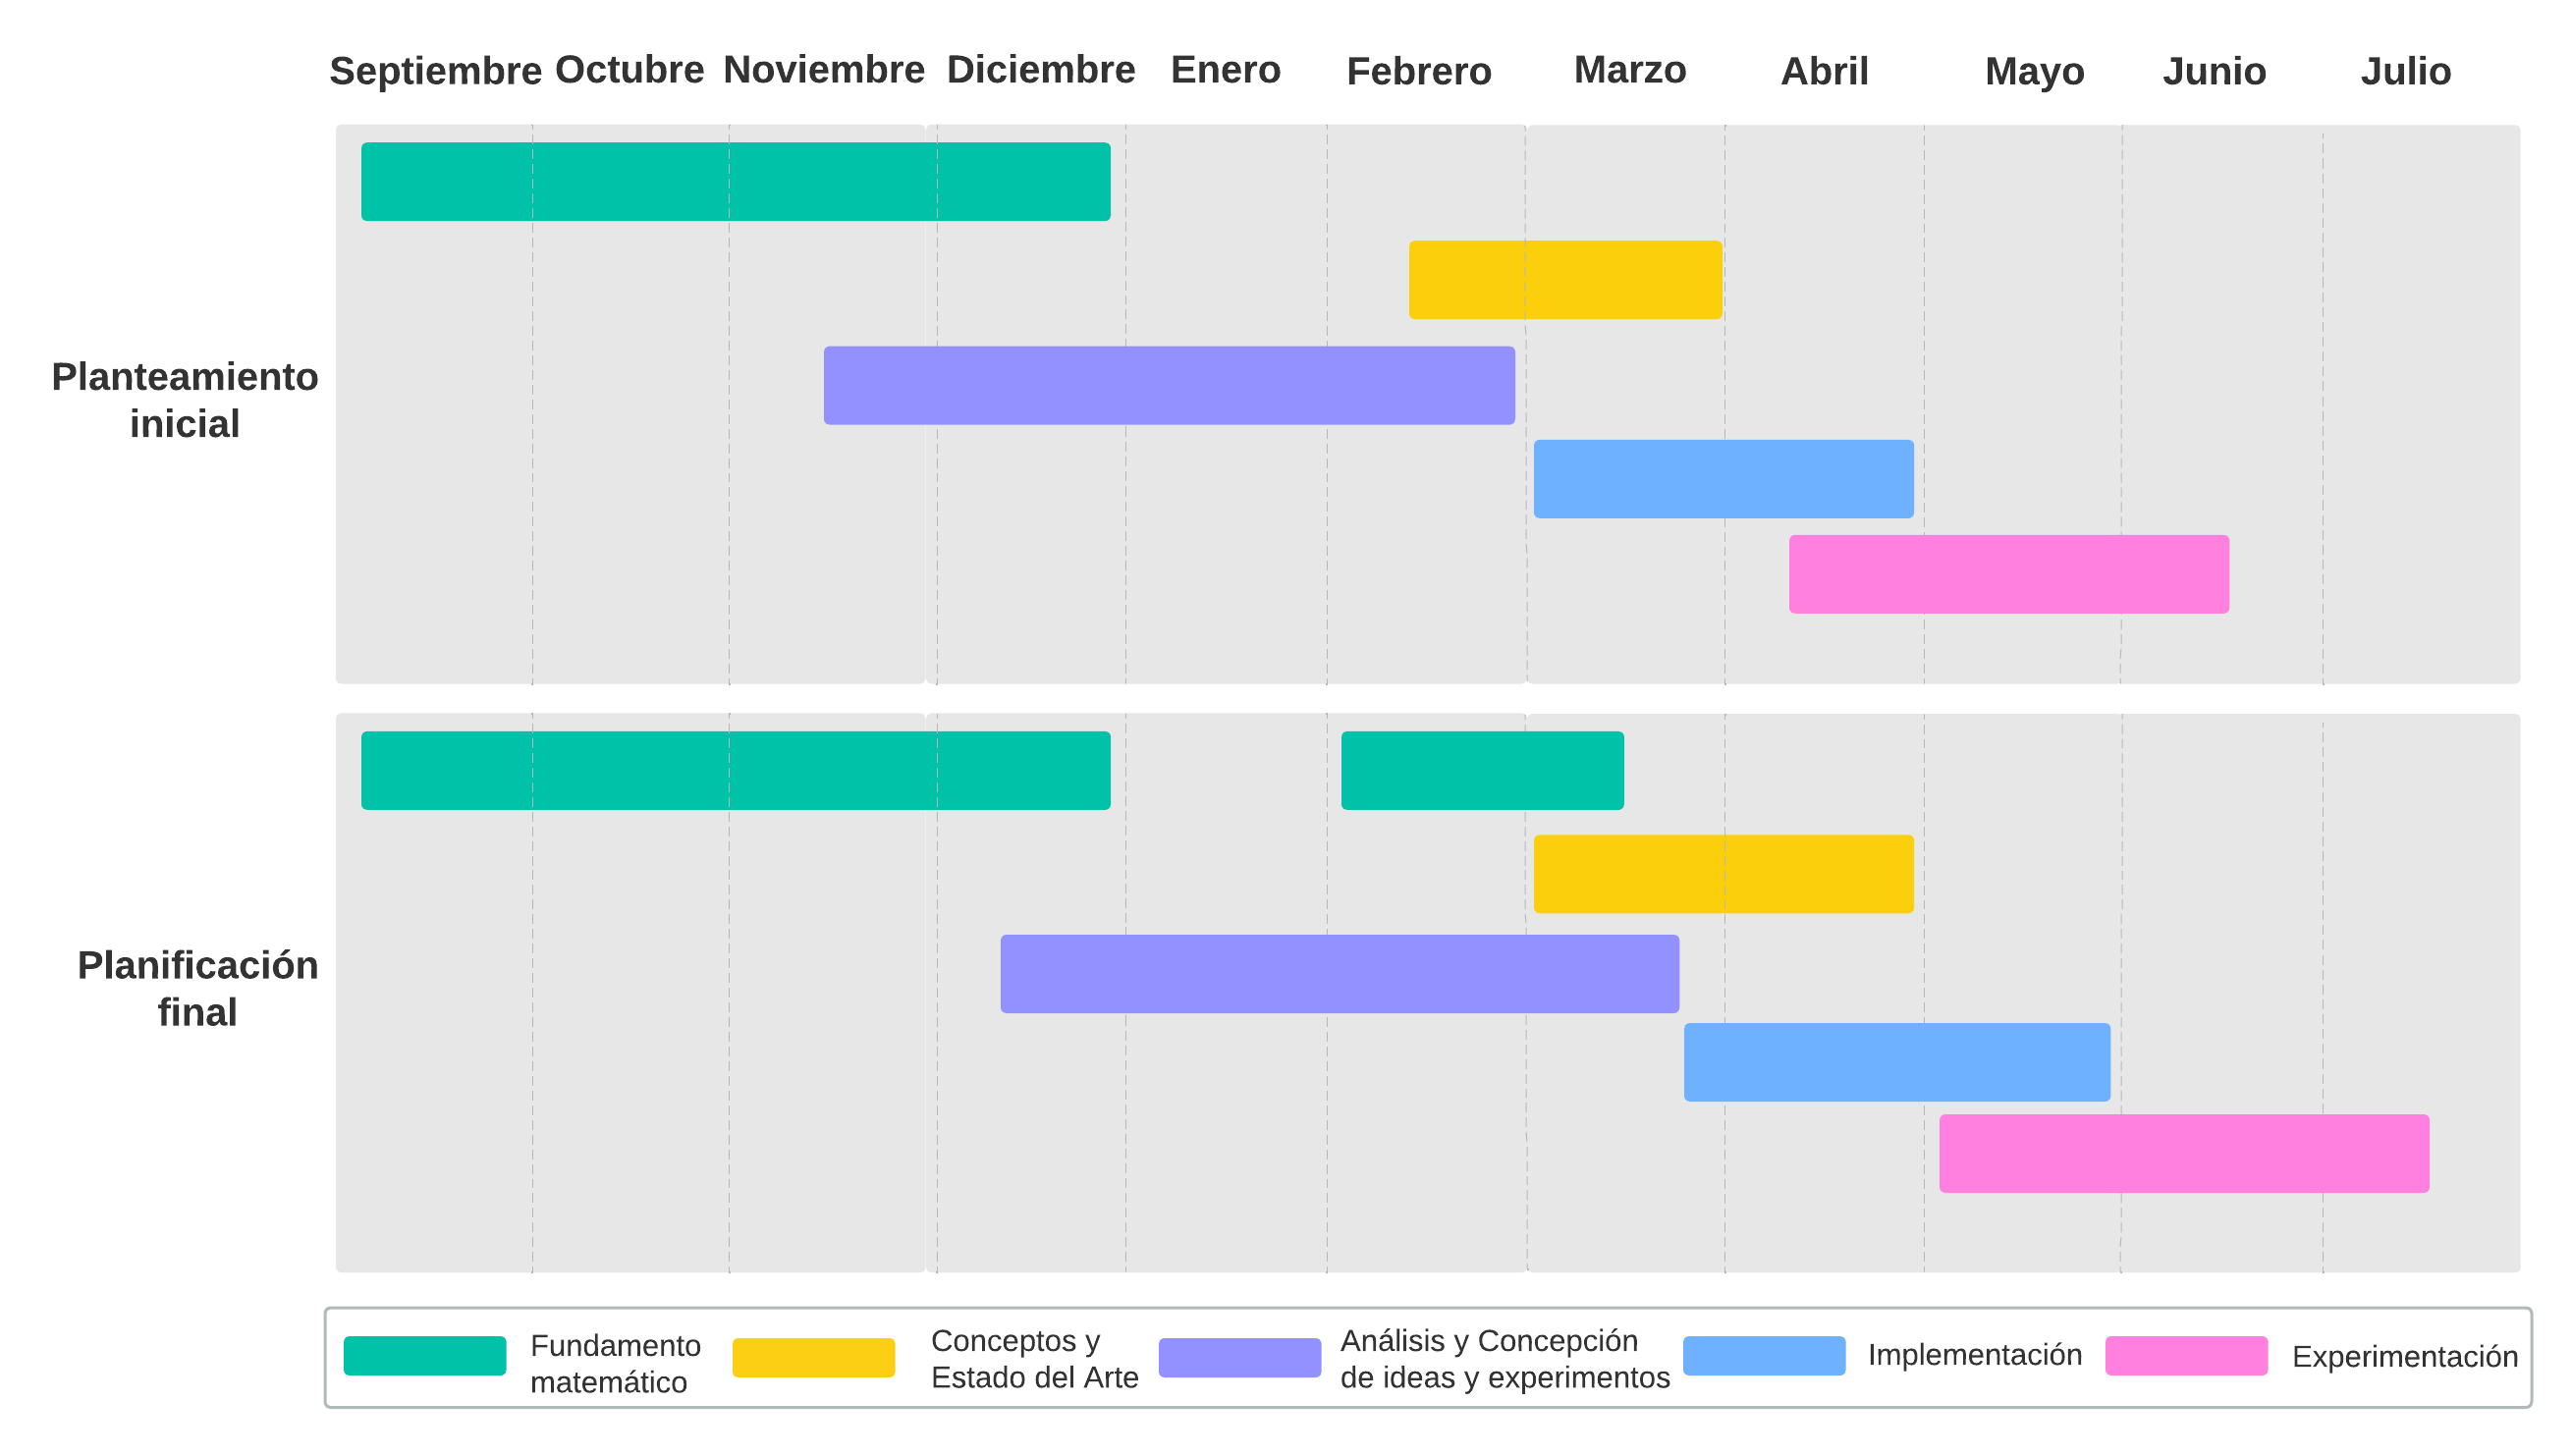
\includegraphics[width=150mm]{img/planificacion.png}
	\caption{Planificación temporal prepuesta frente a la finalmente realizada.}
	\label{fig:plan}
\end{figure}

\endinput